
\documentclass{VUMIFPSkursinis}
\usepackage{algorithm}
\usepackage{algpseudocode}
\usepackage{amsfonts}
\usepackage{amsmath}
\usepackage{bm}
\usepackage{caption}
\usepackage{color}
\usepackage{float}
\usepackage{graphicx}
\usepackage{listings}
\usepackage{longtable}
\usepackage{url}
\usepackage{subfig}
\usepackage{wrapfig}
\usepackage{algorithmicx}
\graphicspath{ {img/} }
\usepackage{rotating}
\usepackage{enumitem}

% Titulinio aprašas
\university{Vilniaus universitetas}
\faculty{Matematikos ir informatikos fakultetas}
\department{Programų sistemų katedra}
\papertype{Kursinis darbas}
\title{Pakartotinis kodo panaudojimas pirminio kriptovaliutų platinimo išmaniuosiuose kontraktuose}
\titleineng{Code Reuse in Initial Coin Offering Smart Contracts}
\status{3 kurso 1 grupės studentė}
\author{Agnė Mačiukaitė}
\supervisor{lekt. Gediminas Rimša}
\date{Vilnius \\ \the\year}


\bibliography{library} 

\begin{document}

\maketitle

\tableofcontents


\sectionnonum{Įvadas} \label{ivadas}

Kodo pernaudojimas leidžia naudoti programas keliuose projektuose. Tai yra svarbi strategija kodui, norint padidinti sistemos efektyvumą ir kokybę. Taikant pernaudojamumą programuotojai naudojasi jau įgyvendintu kodu, kurį keičia taip, kad jis atitiktų naujo projekto reikalavimus \cite {Ravichandran2003}. Viena iš būtinų sąlygų, kuriant pernaudojamą kodą yra supratimas skirtingų kontekstų, kuriuose pernaudojamas kodas galėtų būti naudojama ir kaip būtų valdomas jo pernaudojamumas. Tai padeda programuotojams nuspręsti ar kodas atitinka reikalavimus ir gali būti kuriamas, jei taip, tai ką reikia parametrizuoti ir kaip struktūrizuoti kodą, kad vėliau būtų galima ją pritaikyti skirtingiems kontekstams \cite{Kang1990}.

Pirminio kriptovaliuto platinimo (angl. initial coin offering, toliau ICO) metu įmonė parduoda specializuotus kripto-žetonus žadėdami, kad žetonai veiks kaip mainų priemonė gaunat paslaugas įmonės platformoje. Žetonų pardavimas kuria kapitalą pradiniam įmonės platformos kūrimui, nors nėra įsipareigojimo dėl būsimos paslaugos kainos (žetonais ar kitaip). Neseniai iškylęs ICO populiarumas yra paveiktas Bitcoin ir Ethereum sukurtos kriptovaliutos su papildoma programavimo galimybe \cite{Catalini2018}. Ethereum ir Bitcoin šiuo metu dvi populiariausios blokų grandinės (angl. blockchain, toliau blockchain) \cite{Luu}. Bitcoin - skaitmeniniai pinigai, kurių pavedimai vyksta internete naudojantis decentralizuota vieša duomenų baze - blockchain \cite{Swan2015}. Ethereum be savo kriptovaliutos turi ir kitą svarbų funkcionalumą - išmaniuosius kontraktus - Turing complete programą, kuri leidžia rašyti decentralizuotas aplikacijas \cite{Buterin2014}. Solidity - populiariausia kalba, naudojama rašyti išmaniesiems kontraktams \cite{Dannen}. Problema - išmaniųjų kontraktų technologijos yra pakankamai jaunos, dėl to pakartotinio kodo panaudojimo bazė dar tik formuojasi. Šiuo metu ICO išmanieji kontraktai yra tiražuojami kopijavimo su modifikacijos būdu.

Produktų linijos programinė įranga (angl. product line software engineering, toliau PLSE) naudojama įmonėse pakartojamumui susijusiuose programinės įrangos produktuose numatyti. PLSE suteikia bendrą architektūrą ir pernaudojamą kodą programinės įrangos kūrėjams \cite{Svahnberg}. Toks kūrimas susideda iš savybių išskyrimo ir jų įgyvendinimo produkte. Gerai išskirtos produkto ypatybės padeda sukurti lengvai pernaudojamą programą. Savybės turi būti atrinktos atsižvelginat į jų paplitimą bei kintamumą srityje \cite{Lee2015}. Naudojantis PLSE produkto kūrėjai gali fokusuotis produkto specifikacijoje, o ne bendrose savybėse \cite{Svahnberg}.

Savybių modeliavimas yra pagrindinis metodas atrinkti bei valdyti bendrąsias ir kintamas savybes produktų linijoje. Programinės įrangos šeimos gyvavimo pradžioje savybių modelis padeda išskirti pagrindines savybes, kurios gelbsti kuriant naują rinką ar  norint išlikti jau esamoje. Taip pat savybių modelis leidžia išskirti rizikingas savybes, nuspėti, kokia yra visos programos ar atskirų savybių kaina. Vėliau savybių modeliavimas padeda išskirti variacijos taškus programinės įrangos architektūroje \cite{Czarnecki2004}. Savybių modeliavimas yra populiariausias PLSE kūrime nuo pat pirmojo jo pristatymo \cite{Kang1990}. Kadangi savybės yra pakankamai abstraktus konceptas, padedantis efektyviai bendrauti suinterasuotoms šalims. Savybių modeliavimas yra intuityvus ir efektyvus būdas, žmonėms išreikšti savybių paplitimą ir kintamumą programinės įrangos šeimoje \cite{Kang2013}. 

Šio darbo tikslas - ištirti pirminio finansavimo kriptovaliutomis išmaniuosius kontraktus, nustatyti, kokios savybės yra pastavios, o kokios - kintamos bei pasiūlyti būdus kodo pernaudojamumui didinti. 

Tikslui pasiekti išsikelti uždaviniai:
\begin{enumerate}[topsep=0pt,itemsep=-1ex,partopsep=1ex,parsep=1ex]
\item Apžvelgti savybių modeliavimą programinės įrangos produktų linijos sričiai;
\item Surinkti virš 100 išmaniųjų kontraktų skirtų ICO;
\item Išskirti surinktų išmaniųjų kontraktų savybes;
\item Sukurti ICO savybių modelį ir jį validuoti.
\end{enumerate}

\section{Savybių modeliavimas}

Savybių modeliavime bendri ir kintami bruožai yra modeliuojami iš produkto savybių perspektyvos PLSE. Originalus savybių modeliavimas - FODA (angl. Feature-Oriented Domain Analysis (FODA), toliau FODA) \cite{Kang1990} - paprastas modelis, kuris savybes skirsto pagal „susideda iš" santykį bei pagal bendrumą ir specializaciją naudojant IR/AR (angl. AND/OR)  diagramas. Savybės yra suskirstytos į būtinas, alternatyvias ir pasirenkamas pagal bendrus ir kintamus bruožus \cite{Kang2013}.

\subsection{Savybė} \label{savybe}

Keli tos pačios srities programinės įrangos produktai turi daug bendrų galimybių, bet taip pat kiekviena programinė įranga turi ir savo išskirtinumų. Tos galimybės iš naudotojo perspektyvos yra savybės \cite{Kang1990}. Savybės yra pagrindinis produkto skiriamasis bruožas. Skirtingi srities analizės metodai terminą savybė apibūdina šiek tiek kitaip \cite{Lee2015}. FODA \cite{Kang1990} savybę apibūdina kaip pastebimą ir skiriamą sistemos charakteristiką, kuri yra matoma įvairioms suinteresuotoms šalims.

FODA fokusuojasi ties kliento perspektyva, tai yra ties paslaugomis, kurias teikia aplikacija ir aplinka, kurioje dirbama. Savybės yra programinės įrangos atributai, kurie tiesiogiai paveikia naudotoją \cite{Kang1990}. Skirtumas tarp savybės ir konceptualios abstrakcijos (pvz.: funkcijos, objekto) yra tai, kad funkcijos ir objektai yra naudojami specifikuojant vidines programinės įrangos detales. Kitaip, funkcijos ir objektai yra konceptualios abstrakcijos, kurios yra identifikuojamos iš vidinės programinės įrangos pusės. Savybė - aiškiai matoma  pagal charakteristiką, kuri gali išskirti produktą iš kitų. Todėl savybių modeliavimas turi išskirti iš išorės matomas charakteristikas produktuose bendrumo ir kintamumo atžvilgiu, o ne apibūdinti visas produkto modeliavimo detales (pvz.: funkcinis, objektais orientuotas modeliavimas). Suprantant produkto bendrus ir kintamus bruožus galima sukurti pernaudojamas funkcijas ir objektus \cite{Lee2015}.

\subsection{Savybių modelis}

FODA \cite{Kang1990} autoriai apibrėžia savybių modelį, kaip modelį, kuris turi pavaizduoti standartines sistemos šeimos savybes srityje ir santykius tarp jų. Trumpiau - savybių modelis yra hierarchiškai išskirstytų savybių rinkinys - „susideda iš" santykių rinkinys \cite{Kang1990, Batory2005}. Santykiai tarp savybių  modelyje yra kategorizuojami į ( \ref{img:fm_rules} pav.):
\begin{itemize}[topsep=0pt,itemsep=-1ex,partopsep=1ex,parsep=1ex]
\item Ir - visos vaikinės savybės turi būti pasirinktos;
\item Alternatyva - tik viena vaikinė savybė gali būti pasirinkta ;
\item Ar - viena ar daugiau gali būti pasirinkta;
\item Privaloma - savybė yra privaloma;
\item Pasirenkama - savybė gali būti pasirenkama.
\end{itemize}

\pagebreak

\begin{center}
    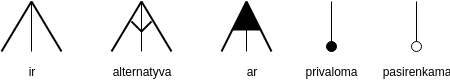
\includegraphics[scale=0.75]{img/feature_model_rules}
    \captionof{figure}{Santykių kategorijos tarp savybių \cite{Batory2005}}
    \label{img:fm_rules}

\end{center}

Savybių diagrama yra grafinė savybių modelio reprezentacija. Tai modelis - medis, kur primityvios savybės - lapai, pagrindinės - mazgai (modelio pavyzdys - \ref{img:fm_example} pav.). Būtinos savybės tarp skirtingų produktų yra modeliuojamos kaip privalomos, kai skirtingos savybės tarp jų žymimos kaip alternatyvios ar pasirenkamos (angl. optional) \cite{Batory2005}. Bendros savybės atributai yra paveldimi pagal visą jos specifikaciją. Visos pasirenkamos ar alternetyvios savybės, kurios negali būti pasirinktos, kai yra bendra savybė pasirinkta turi būti pažymėtos kaip tarpusavyje nesuderinamos (angl. mutually exclusive with). Visos pasirenkamos ir alternatyvios savybės, kurios turi būti pasirinktos, kai bendra yra pasirinkta, turi būti pažymėtos kaip privalomos. Savybių modelio dokumentacija susideda iš stuktūrinės diagramos hierarchiškai suskaidančios savybes indentifikuojančias pasirenkamas ir alternatyves savybes, savybių apibūdinimo ir taisyklių kompozicijos savybėms \cite{Kang1990}. 

\begin{center}
    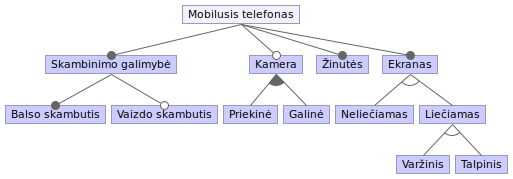
\includegraphics[scale=0.6]{img/mobile}
    \captionof{figure}{Savybių modelis mobiliajam telefonui \cite{Kang2013}}
    \label{img:fm_example}
\end{center}

Pasirenkamos ir alternatyvios savybės negali būti atrinktos savavališkai. Įprastai jos parenkamos pagal galutinio naudotojo (kliento) tikslus ar interesus \cite{Kang1990}. Labai naudinga yra tai, kad savybė yra efektyvus komunikavimo būdas tarp suinteresuotų šalių. Dažnai klientai ir inžinieriai kalba apie produkto charakteristiką savybių pavidalu. Reikalavimai ir funkcijos yra apibūdinami kaip savybės, kadangi jos yra aiškiai atpažįstamos abstrakcijos (plačiau \ref{savybe}. Savybė) \cite{Lee2015}. Savybių modelis taip pat tarnauja kaip komunikacija tarp naudotojų ir kūrėjų. Naudotojui savybių modelis teikia informaciją, kokios yra savybės, iš kurių gali rinktis ir kada. Kūrėjams savybių modelis identifikuoja, ką reikėtų parametrizuoti kituose modeliuose bei programinės įrangos architektūroje ir kaip parametrizacija turi būti atlikta \cite{Kang1990}. Kitaip, savybių modelis gelbsti ne tik pernaudojamų komponentų kūrime, bet ir valdant produktų konfigūraciją srityje \cite{Lee2015}.

%Srities savybių modelis ir programinės įrangos architektūra turi būti apibrėžta aplink standartines savybes. Alternatyvios ir pasirenkamos savybės turi būti įtrauktos į modelį ir arcihtektūrą, bet visada turi būti parametrizuotos su atitinkamomis savybės, kad įsikyšimas į modelį ir architektūra būtų nesudėtingas \cite{Kang1990}. 


\subsection{Procesas ir gairės} \label{procesas}

Savybių analizė susideda iš reikalingų dokumentų surinkimo, savybių išskyrimo, savybių abstrakcijos ir identifikavimo modelyje, savybių apibrėžimo, modelio validacijos \cite{Kang1990}. Tačiau, prieš atliekant savybių modelį pirma turėtų būti išskirta sritis, kurios savybių analizė bus atliekama \cite{Lee2015}. 

\subsubsection{Srities identifikavimas}

Srities identifikavimas prasideda nustantant sritį su kuria bus dirbama. Pasirinkus sritį turi būti nubrėžtos ribos ir santykiai tarp srities elementų ir kitų esybių, esančių už srities ribų bei informacijos dalinimasis vieni tarp kitų. Srities modeliavimo tikslas yra nustatyti bendrus ir skirtingus konceptus ar charakteristikas sistemos kūrime \cite{Lee2015}.  

\subsubsection{Savybių identifikavimas} \label{identifikavimas}

Savybių identifikavimas susideda iš išskyrimo srities žinių gautų iš srities ekspertų ir kitų dokumentų tokių kaip knygos, nadotojo vadovo, projektavimo dokumentų ir jau parašytų programų \cite{Lee2015}. Aplikacijos savybes galima išskirti į keturias kategorijas:
\begin{itemize}[topsep=0pt,itemsep=-1ex,partopsep=1ex,parsep=1ex]
\item darbo aplinka, kurioje aplikacijos yra naudojamos;
\item galimybės iš naudotojo perspektyvos;
\item srities technologija - kokiais reikalavimais remiantis sprendimas yra padaromas;
\item įgyvendinimo technika.
\end{itemize}

%Metodas fokusuojasi ties savybėmis susijusiomis su aplikacijos galimybėmis. 

%Galimybių savybės dar gali būti suskirstytos į:
%\begin{itemize}
%\item funkcines
%\item operacines
%\item pateikimo (prezentacijps)
%\end{itemize}

%Funkcinės savybės yra servisai, kurie yra suteikti aplikacijos. Tokios savybės gali būti rastos naudotojo vadove bei reikalavimų dokumentacijoje. Operaicnės savybes - tos kurios susiję su aplikacijos operacijomis (taip pat iš vartotojo perspektyvos); tai yra, kaip naudotojas sčveikauja su aplikacija. Naudotojo vadivas yra geras tokių savybių šaltinis. Prezentacijos - tai kaip ir kokia informacija yra pateikama naudotojui. Tokia informacija randama naudotojo vadove ir reikalavimų specifikacijoje. 

Visos identifikuotos savybės turi būti pavadintos ir konfliktai susiję su vardais turi būti išspręsti. Savybių sinomimai taip pat turi būti įtraukti į srities terminologijos žodyną \cite{Kang1990}.

\subsubsection{Savybių abstrakcija, klasifikacija, modeliavimas}

Sekantis žingsnis identifikavus savybes turėtų būti hierarchinio modelio sukūrimas pagal savybių klasifikavimą, strūkturizavimą naudojant „susideda iš" santykį. Ar savybė yra būtina, alternatyvi, pasirenkama turi būti identifikuojama modelyje. Kiekviena savybė modelyje turi būti apibrėžta \cite{Kang1990}.

\subsubsection{Savybių modelio validacija} \label{validacija_teor}

Ar savybių modelis gerai reprezentuoja srities savybes turi būti validuota prieš srities ekspertus ir  jau egzituojančias aplikacijas. Srities ekspertai, kurie konsultavo analizės metu, neturi dalyvauti validacijoje. Taip pat bent viena aplikacija, kuri nebuvo naudota analizėje, turi būti panaudota, kad  būtų nustatytas modelio bendrumas ir pritaikomumas. Jei įmanoma validuojant turi būti panaudotas naujas aplikacijų rinkinys \cite{Kang1990}.
 


\section{Savybių modeliavimas ICO išmaniesiems kontraktams}

Buvo pasirinkta atlikti savybių modeliavimą remiantis procesu aprašytu \ref{procesas}. skyriuje. Savybių modeliavimas buvo pradėtas nuo srities nusistatymo (plačiau \ref{sritis}. Srities identifikavimas), tada buvo surinkta informacija reikalinga srities modelio sudarymui ir savybių išskyrimui bei atrinktos savybės (plačiau \ref{isskyrimas}. Savybių identifikavimas), sekantis žingsnis buvo modelio sudarymas (plačiau \ref{modelis}. Savybių modelis) ir jo validacija (plačiau \ref{validacija}. Savybių modelio validacija).

\subsection{Srities identifikavimas} \label{sritis}

Šio savybių modeliavimo sritis - išmanieji kontraktai pirminiam kriptovaliutų platinimui. Kaip jau buvo minėta\ref{ivadas} įvade: „Išmaniųjų kontraktų technologijos yra pakankamai jaunos, dėl to pakartotinio kodo panaudojimo bazė dar tik formuojasi. ICO kontraktai yra tiražuojami kopijavimo su modifikacijos būdu." Todėl šiame savybių modeliavime bus apsirobojama tik ICO naudojamais kontraktais ir nebus analizuojami santykiai su kitais išmaniaisiais kontraktais ar sistemomis.


\subsection{Savybių identifikavimas} \label{isskyrimas}

Savybių modelio sukūrimui yra būtinas savybių identifikavimas. Remiantis \ref{identifikavimas}. skyriuje aprašytu savybių identifikavimo būdais buvo pasirinktas jau parašytų programų (šiuo atveju išmaniųjų kontraktų) surinkimas, analizavimas ir savybių juose identifikavimas. Išmaniųjų kontraktų surinkimo procesas:
\begin{enumerate}[topsep=0pt,itemsep=-1ex,partopsep=1ex,parsep=1ex]
\item Iš Ethereum blockchain blokų naršyklės - etherscan.io\footnote{\url{https://etherscan.io/}}, buvo atrinkti išmaniųjų kontraktų adresai ir nuorodos į juos platformoje;
\item Parašytas interneto skaitytuvas\footnote{Interneto skaitytuvas patalpintas: \url{https://github.com/maciukaite/kursinis/tree/crawler-etherscan}} (angl. web crawler) naudojantis Node.js karkasu;
\item Visi surinktų išmaniųjų kontraktų kodai buvo surašyti į failus\footnote{Visi failai patalpinti: \url{ https://github.com/maciukaite/kursinis/tree/crawler-etherscan/res}}. Failo pavadinino struktūra: contract + identifikacijos numeris + .sol plėtinys;
\end{enumerate}

Tokiu būdu buvo surinkta 128 pirminio kriptovaliutų platinimo išmanieji kontraktai. Savybės iš išmaniųjų kontraktų buvo išskirtos analizavimo būdu - pirmiausia atrinkta 21 išmanusis kontraktas, kuris neturi savybės - žetono sukūrimas ir disponavimas (priežastys šiam pasirinkimui yra pateiktos \ref{sritis} skyriuje). Išanalizavus atrinktus kontraktus buvo išskirtos savybės ir apibūdintos dalinai naudojantis forma pateikta FODA \cite{Kang1990}:

\pagebreak

\begin{center}
    \captionof{table}{Atrinktos aibės ICO išmaniųjų kontraktų savybės}
    \begin{longtable}[H]{| p {5cm} | p{5cm} | p{5cm} |}
    \hline
    \textbf{Savybės pavadinimas } &\textbf{Apibūdinimas} & \textbf{ICO išmaniųjų kontraktų numeriai} \endhead \hline
	
	Žetono kainos nustatymas skirtingomos pakopomis  & ICO metu žetonas gali turėti kelias kainas, skirtinga pakopa žetonų platinime - skirtinga kaina  & 2, 23, 43, 46, 55, 62, 85, 120
 \\ 
	\hline
	
	
	Minimalaus investavimo kriterijus & Naudotojas turi būtinai ivestuoti sumą nemažensę nei 15  & 2, 16, 46, 106  \\ 
	\hline
	
	ETH susigrąžinimo galimybė nepasiekus tikslo & Jei ICO nepasiekia nusistatyto minimalaus suinvestuotų pinigų ribos, tai visi investuoti pinigai yra grąžinami naudotojams  & 2, 23, 46, 62, 85, 94, 96, 120  \\ 
	\hline
	
	Žetonų atsiėmimas tik įvykus ICO & Įvykus ICO naudotojai gauna nusipirktus žetonus  & 2, 126 \\ 
	\hline
	
	Kainos už žetoną pakeitimas & Žetono kaina gali kisti neatsižvelgiant į pasikeičiančias pakopas  & 2, 40  \\ 
	\hline
	
	Kontrakto savininko nustatymas bei kai kurio funkcionalumo priskyrimas tik jam & Išmanusis kontraktas turi priviligijuotą adresą - kontrakto savininką, kuris turi daugiau funkcionalumo nei įprastas naudotojas  & 2, 12, 13, 16, 23, 31, 43, 46, 62, 72, 85, 86, 94, 106, 114, 116, 120, 126 \\ 
	\hline
	
	Galimybė sustabdyti ICO ir vėl paleisti iš naujo & ICO sustabdymo metu nebūtų galima nusipirkti žetonų  &  12, 31\\ 
	\hline
	
	Galimybė pirkimo metu nustatyti kitą adresą kaip pirkėją & Naudotojas pirkdamas žetonus nustato adresą (pirkėją), kurį atstovauja  & 12, 31, 62  \\ 
	\hline
	
	Pirkimas tik indentifikuotiems naudotojams & Pirkti žetonus gali tik anksčiau į išmaniajame kontrakte pažymėti naudotojai  & 12, 16, 31 \\ 
	\hline
	
	ICO sustabdymas ar galimybė keisti datą & ICO galima sustabdyti ar keisti jo pabaigos datą  & 16, 43, 46, 86, 106  \\ 
	\hline
	
	Pelno pasiskirstymas tarp komandos ir įmonės & Surinkta pinigų suma yra paskirstyta ne tik įmonei, bet ir komandai  &  23\\ 
	\hline
	
	ICO pradžios nustatymas  & ICO pradžios data gali būti keičiama  &  40, 86, 106, 126 \\ 
	\hline
	
	
	Maksimalaus galimo surinkti ETH keitimas & Galimybė papidinti ar sumažinti investicijų sumos skaičių  & 43, 86 \\ 
	\hline
	
	Nustatytas maksimalus galimas žetonų kiekis nupirktas per kartą & Naudotojas gali nusipirkti ne daugiau žetonų nei yra nustatyta  & 43 \\ 
	\hline
	
	Nereikalingų žetonų išsitraukimas iš kontrakto  & Likusių žetonų nuo ICO susigrąžinimas  & 13, 62, 94, 114, 120, 126 \\ 
	\hline
	
	Žetonų išskyrimas komandai & Žetonų paskirstymas komandos nariams  &  62, 72, 94, 114, 120, 126\\ 
	\hline
    \end{longtable}
	\addtocounter{table}{-1}

    \label{table:features}

\end{center}



\subsection{Savybių abstrakcija, klasifikacija, modeliavimas} \label{modelis}

Savybių modelis ICO išmaniesiems kontraktams (\ref{img:fm_ico} pav.) buvo sudarytas naudojantis savybėmis, kurios yra išvardintos \ref{isskyrimas}. skyriuje, \ref{table:features} lentelėje. Savybių pavadinimai esantys lentelėje ir modelyje gali nesutapti, kadangi savybės modelyje yra padaryta savybių abstrakcija ir kai kurios savybės ar jos dalys yra sujungtos. Jei savybė lentelėje neturėjo sau priešingos, tai modelyje priešinga savybė jau yra įvardinama ir tai priimtina kaip savaime suprantamas reiškinys. Visos savybės buvo klasifikuotos ir struktūrizuotos naudojant „susideda iš" santykį, taip pat savybės modelyje identifikuotos naudojantis santykių kategorijomis tarp savybių (\ref{img:fm_rules} pav.). Modelio kompozicijos taisyklės:
\begin{enumerate}[topsep=0pt,itemsep=-1ex,partopsep=1ex,parsep=1ex]
\item Nereikalingų žetonų susigrąžinimui reikalingas savininkas;
\item Platinimo periodo keitimui reikalingas savininkas;
\item Kainos pakeitimui rankiniu būdu reikalingas savininkas;
\item Žetonus atsiimti po ICO gali tik pirkėjas;
\item ETH susigrąžinti nepasiekus tikslo gali tik pirkėjas.
\end{enumerate}

Savybės, kurios neturi vaikinių savybių, turi identifikacijos numerį, tam, kad validuojant modelį būtų galima lengviau identifikuoti bendras savybes.

\begin{sidewaysfigure}

\begin{center}
    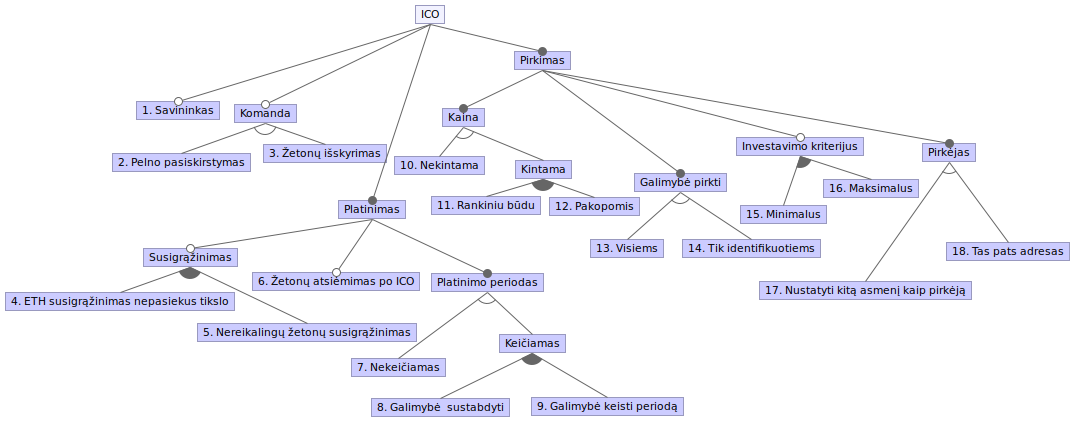
\includegraphics[scale=0.7]{img/ico_model_num}
    \captionof{figure}{Savybių modelis ICO išmaniesiems kontraktams}
    \label{img:fm_ico}
\end{center}

\end{sidewaysfigure}
\pagebreak

\subsection{Savybių modelio validacija} \label{validacija}

Remiantis \ref{validacija_teor}. skyriuje aprašytu procesu validuoti modelį turėtų srities ekspertai ar naujas dokumentų rinkinys. Kadangi šiame darbe negalima pasinaudoti srities ekspertais, tai validacijai naudojami dokumentai - išmanieji kontraktai, kurie buvo surinkti anksčiau (plačiau \ref{isskyrimas}. skyriuje). Iš dar nenaudotų dokumentų buvo atsitiktinai atrinkta 10 išmaniųjų kontraktų ir patikrinta ar savybių modelis (\ref{img:fm_ico} pav.) yra validus. Validacijos rezultatas pateiktas lentelėje:
\begin{center}
    \captionof{table}{ICO savybių modelio validacija}
    \begin{longtable}[H]{| p {3cm} | p{8cm} | p{2.5cm} |}
    \hline
    \textbf{ICO išmaniųjų kontraktų numeriai}  & \textbf{Savybės numeris} & \textbf{Validumas} \endhead \hline
	
	0 & 1, 5, 7, 10, 13, 15, 16, 18
& validus
 \\ 
	\hline
	6 & 1, 7, 10, 13, 15, 18 & validus
	\\
		\hline
	22 & 1, 5, 9, 10, 13, 15, 18 & validus
	\\
		\hline
	33 & 1, 8, 9, 11, 14, 18 & validus
	\\
		\hline
	39 & 1, 4, 8, 9, 10, 13, 15, 18 & validus
	\\
		\hline
	51 & 1, 3, 5, 7, 10, 13, 18 & validus
	\\
		\hline
	71 & 7, 10, 13, 18 & validus 
	\\
		\hline
	91 & 7, 10, 13, 18 & validus
	\\
		\hline
	103 & 1, 8, 9, 10, 14, 15, 16, 18 & validus
	\\
		\hline
	122 & 1, 7, 10, 13, 15, 16, 18 & validus
	\\
		\hline
		
		
\end{longtable}
    \label{table:validacija}

\end{center}


\sectionnonum{Rezultatai ir išvados}

Šiame darbe pasiekti rezultatai:
\begin{enumerate}[topsep=0pt,itemsep=-1ex,partopsep=1ex,parsep=1ex]

\item Apžvelgtos kodo pernaudojimo galimybės naudojantis savybių modeliavimu;
\item Surinkti ICO išmanieji kontraktai bei ištirtos jų savybės;
\item Nustatyta, kurios savybės yra pastovios ir kintamos;
\item Kodo pernaudojamumui didinti sudarytas savybių modelis.

\end{enumerate}

Darbo tikslas - ištirti pirminio finansavimo kriptovaliutomis išmaniuosius kontraktus, nustatyti, kokios savybės yra pastavios, o kokios - kintamos bei pasiūlyti būdus kodo pernaudojamumui didinti - pasiektas.

\bigbreak

Pasiekti rezultatai leidžia daryti išvadas:
\begin{enumerate}[topsep=0pt,itemsep=-1ex,partopsep=1ex,parsep=1ex]
\item Savybių modeliavimas yra geras būdas ICO išmaniųjų kontraktų kodo pernaudojamumui didinti;
\item Yra sukurta pakankamai daug ICO išmaniųjų kontraktų turinčių įvairių savybių, todėl žinant, koks savybių rinkinys yra reikalingas, būtų galima pernaudoti esamą kontraktą ar jo dalį.
\end{enumerate}

\bigbreak

Darbą galima toliau tęsti šiomis kryptimis:
\begin{enumerate}[topsep=0pt,itemsep=-1ex,partopsep=1ex,parsep=1ex]
\item Tobulinti savybių modelį paimant didesnę aibę ICO išmaniųjų kontraktų;
\item Būtų galima ICO savybių modelį panaudoti kuriant ICO išmaniųjų kontraktų produktų liniją. Taip pat sukurti ICO išmanųjį kontraktą, kuris remtusi savybėmis iš modelio bei jau sukurtu kodu ir leistų jais lengvai varijuoti.
\item Būtų galima panaudoti savybių modelį jau sukurtoms išmaniųjų kontraktų bibliotekoms tobulinti.
\end{enumerate}


\printbibliography[heading=bibintoc] % Literatūros šaltiniai aprašomi
%bibliografija.bib faile. Šaltinių sąraše nurodoma panaudota literatūra,
%kitokie šaltiniai. Abėcėlės tvarka išdėstoma tik darbe panaudotų (cituotų,
%perfrazuotų ar bent paminėtų) mokslo leidinių, kitokių publikacijų
%bibliografiniai aprašai (šiuo punktu pasirūpina LaTeX). Aprašai pateikiami
% netransliteruoti.

\sectionnonum{Sąvokų apibrėžimai}
Turing complete - bet kuri sistema, kuri yra pakankamai galinga atpažinti visus galimus algoritmus \cite{Teller1994}. 

Interneto skaitytuvas (anlg. web crawler) -  programa, kuri nuskaito svetainę ar svetainių rinkinį, analizuoja surinktus puslapius ir praneša apie rezultatus. \cite{Thelwall2001}.

\sectionnonum{Santrumpos}
PLSE - produktų linijos programinė įranga (angl. product line software engineering)

ICO - pirminis kriptovaliutų platinimas (angl. initial coin offering)

FODA - Feature-Oriented Domain Analysis \cite{Kang1990}



\end{document}

